\section{代码走出自己的电脑}
\label{sec:deploy-physical}

前面几章里，你已经能从确定的源码版本构建并运行程序。接下来，学长把机器人推过来：“放到车上跑一下吧。”这时候你才发现，\textbf{在自己的电脑上能运行，只是交付的起点}。机器人真正使用的是机载电脑（onboard computer）：程序要在它的处理器和系统上运行，读取它的相机与串口，并在重新上电后按预期工作。你电脑上的文件夹需要先同步到车上，x86 电脑编译的程序也不能直接拿给 ARM 板运行。

我们把准备目标环境、传送代码与配置、在目标机构建或安装、启动并核验结果这一过程称为\textbf{部署（deployment）}。本章先解决一个最实际的问题：怎样操作机载电脑？等连接稳定了，再讨论如何把程序放上去、让它持续运行，并在故障时找回控制权。

\subsubsection{便携屏和键鼠：最直接的入口}

最传统的办法，是给机载电脑接上一块便携显示器，再插 USB 键盘与鼠标。图~\ref{fig:deploy-monitor} 是一块带 HDMI 输入的小屏幕；对机载电脑来说，它就是普通外接显示器。你可以看到开机画面、登录桌面，像操作自己的电脑一样打开终端，网络还没配好时尤其有用。

\begin{figure}[htbp]
  \centering
  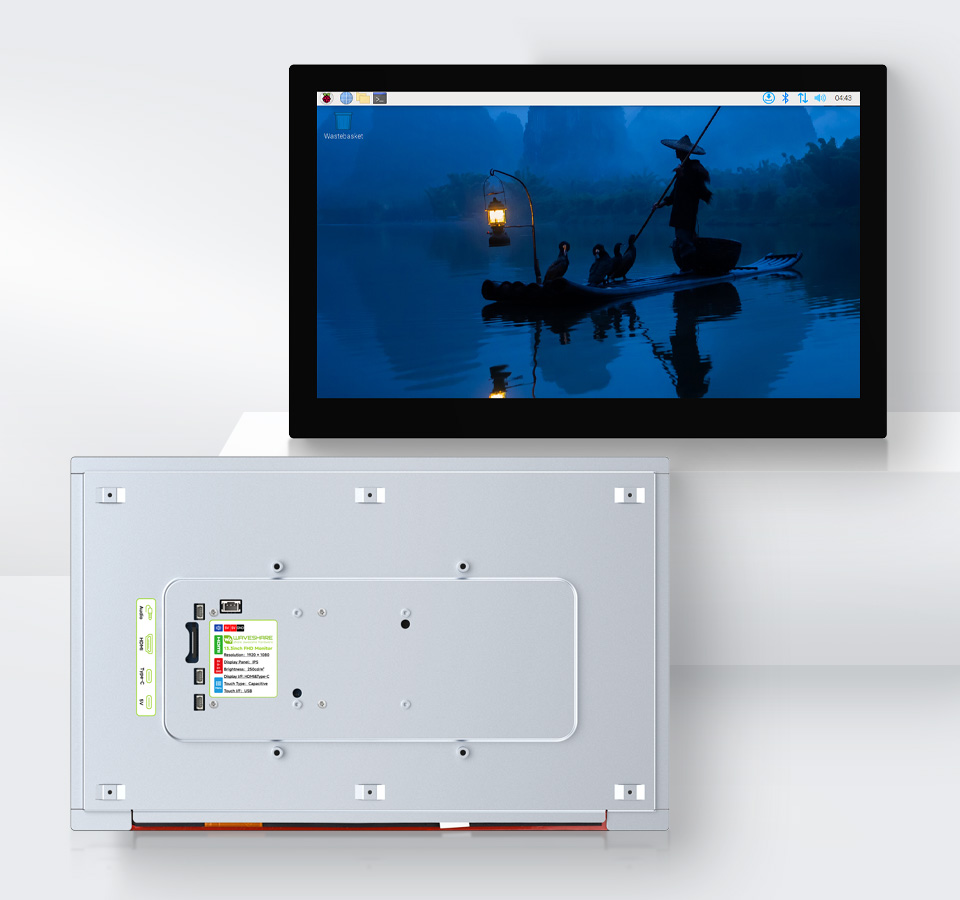
\includegraphics[width=0.58\textwidth]{deployment/portable-monitor.jpg}
  \caption{便携 HDMI 显示器的正反面。先确认视频输入与供电接口，再准备键鼠；图源：Waveshare 官方产品页。}
  \label{fig:deploy-monitor}
\end{figure}

不过，机器人通常不在桌上。你可能一边蹲在地上扶屏幕，一边伸手够键盘，旁边还拖着供电线和视频线；换个位置调车，整套“移动办公桌”又得搬一次。便携屏非常适合首次装机和故障救援，日常开发则可以让自己的笔记本承担键盘与屏幕，把终端或桌面通过连接传回来。接下来的 SSH 和远程桌面，就是为了让你少蹲一会儿。

\begin{example}[首次接入机载电脑]
前提是机载电脑已有可启动的系统，机器人处于队内确认的安全调试状态，不会因为程序误启动产生运动。一定记得注意安全，小心机器人突然甩头把屏幕键盘全部扯到地上，到时候抱着碎掉的便携屏流泪。
先核对电脑的视频\emph{输出}接口与显示器的\emph{输入}接口：HDMI 对 HDMI；只有 DP 输出时，使用方向正确的 DP 转 HDMI 适配器。按显示器铭牌准备电源，再接视频线，最后把有线键鼠插到机载电脑的 USB 口。USB-C 的外形不保证支持视频输出，也不保证能为屏幕供电，应查看两端说明书。

开机后在屏幕上选择对应输入源，确认能看到启动或登录画面。进入桌面后打开终端，运行下面两条只读命令，记录用户名与主机名；后文以用户 \texttt{rm}、主机名 \texttt{rm-robot} 为例，实际使用时换成自己的。
\begin{tbash}
whoami
hostname
\end{tbash}
如果屏幕显示“无信号”，先检查输入源、线材方向与供电，再看主机是否实际启动；此时还没进入 SSH，修改网络配置通常帮不上忙。
\end{example}

\begin{exercise}\label{ex:deploy-physical}
给队内一台机载电脑画出便携屏、屏幕电源与 USB 键鼠的接线图，标明输入和输出方向。接入后记录实际用户名、主机名以及视频接口；没有设备时先按型号手册完成接线方案，现场验证留到本章验收。
\end{exercise}

教材选图用于认识便携屏的外观，大家自行购买合适的便携屏。
